\chapter{Geoid Height Determination Using GeoidApp}
\label{Chapter4}


\section{Introduction}
In this chapter we will discuss the computation of the geoid height and the validation of our results based on local terrestrial data. High resolution models are required to convert GPS leveling data (ellipsoidal height) into orthometric height. For evaluation purposes we have two terrestrial data 1) Astrogeodetic data provided by \cite{osman}, and 2) GPS leveling data by \cite{ahmed_msc}. Our results show higher degrees will often result in a lower standard deviation, i.e., better results. But that should does not always holds true, hence the our evaluation was done using different degrees.
\\
Combined models e.g., EGM2008, EIGEN-6C4, and GECO have a very similar trend--it is expected because both EIGEN-6C4 and GECO share some degrees with EGM2008. Interestingly, ITU\_GGC16, the best model with an error of $0.3653m$ in 149 degree, has the worst results for degrees > 154. Our comparsion with the previous works \citep{ahmed_msc, fashir, godah} shows that our choosen models has surppased them all. For recent works \citep{ahmed_msc, godah}, we show that our model can contribute to their suggested datums of to 40\% (37\% for \citep{ahmed_msc}, and 43 \% for \citep{godah}).



\section{Computing the Geoid}

We developed a software application called GeoidApp for this task. GeoidApp is a huge suite of applications to not only compute geoid height (in addition to gravity anomaly and gravity disturbance), but it also has analysis and interactive visualization features to help the users get the most out of it. For that reason we will discuss the core features about GeoidApp. To compute the geoid height you need to account for these details

\begin{itemize}
	\item The data. GGMs are provided as *.gfc files from ICGEM. They contains in addition to the coefficients text contents about the authors, acknowledgments, etc. They also include model parameters, such as the maximum degree, the model name, the GM, and a few others. The idea is to store the coefficients in an array (for computations efficiency). 
	\item Helper functions for Associated Legendre Polynomials. That could tricky, solving Legendre function is non-trivial. The recursive version of Legendre function is suitable for programming environment.
	\item The main function for geoid computations. You have to choose whether you want to work on point mode, grid mode.
\end{itemize}

\subsection{Working with GGMs data}

Typical GGMs provided by ICGEM are raw and need to be parsed to extract the model's coefficients and other useful informations about the model. When we say a `patter', or `template' we mean that there are certain keywords in the *.gfc files, and it is available in all models.

\subsubsection{Parsing the data}
A typical model from ICGEM would consist of the following

\begin{itemize}
	\item {General information about the mission}. 
	\item {A header with structured details about the models, and their parameters}
	\item {The coefficients part. Which is the core part of the *.gfc files}
\end{itemize}

	\paragraph{Model's summary}. It includes summary about the mission its release date, mission time, etc. There is also a link for detailed informations about the mission. You can safely ignore this part of of the *.gfc file. This part of *.gfc files does not follow any pattern, you cannot build a generic tool to extract informations from it.
	\paragraph{The header}. This summarizes the previous in a template way. It will begin with the keyword \textit{original header}. Below it, there is the name of the model, and the release date, mission duration. It also has information about GM but you can also ignore it here as it will be provided later in more structured way. A good way to think of *.gfc files is xml format. xml files are constructed as \lstinline|<begin_of_tag> some_data </end_of_tag>|. For our work, we treated *.gfc files as follows
	\begin{lstlisting}
	<begin_of_head>
		<original header>
		"product_type": "gravity_field" /* In our case we need this */,
		"model_name": "model_name",
		"radius": "6378136.30" /* It varies over models */,
		"earth_gravity_constant": "398600.4415D+09" /* It varies over models */,
		"max_degree": "n",
		"errors": "formal", /* It could take other values */,
		"tide_system": "tide_free" /* other types are available */,
		</original header>
	</end_of_head>
	\end{lstlisting}
	
	Note that we use those keywords to store these variables with their corresponding values in a data structure (a dictionary, or hash table is suitable for this purpose).
	
	The last part of parsing GGM files is extracting the model coefficients $C_{nm}, S_{nm}$. We want to construct a $(n \times n)$ matrix, where $n$ denotes the maximum degree of our model. For each raw of our matrix will correspond to the degree of the model. Each will have no-zero elements as the index of of that raw. The first raw will always have value 1, and the rest of it are zeros. The second raw will depend on an argument that is specified by the user \textit{subtract\_normal\_field}. In our evaluations we always set such that the ``normal\_field" will be subtracted from coefficients $c_{nm}(1:9,1:9)$. It's important to note that indexing for global geopotential models starts from zero as oppose of one. You should account for that if your are using programming language that uses one as a base for indexing e.g., MATLAB/Octave or Julia.
	
	\(
	C_{nm} = \begin{bmatrix}
		1 & \ldots & \ldots& N_{max}\\
		0 & 0 & \dots & N_{max}\\
		\vdots &\vdots &\ddots & N_{max}\\
		-4.84e-04 & -3.98e-10 & 2.43e-06 & N_{max}\\

	\end{bmatrix}
	\)
	
	For the $S_{nm}$ part there the first column of it, i.e., the value of $S_{nm}$ coefficients are always zero. That is $S_{nm}[:, 0] = 0$. Unlike $C_{nm}$ the number of non-zero elements for each raw in $S_{nm}$ equals the index of that raw minus 1.
	
	\(
		S_{nm} = \begin{bmatrix}
		0 & \ldots &\ldots & N_{max}\\
		0 & 0 & \dots & N_{max}\\
		\vdots &\vdots &\ddots & N_{max}\\
		0 &  1.42e-09& -1.40e-06 & N_{max}\\
		
		\end{bmatrix}
	\)
	

	The same was applied to construct $e_{C_{nm}}, e_{S_{nm}}$ the std values for $C_{nm}, S_{nm}$, respectively.


\section{Software Implementation}
\subsection{Associated Legendre Function}

Solving Legendre function is not easy. It is always good to build on top of others projects, and reference them as needed. We found a few libraries that solve Legendre function. One of them is legendre function in provided by MATLAB. This function does not come with the standard version of MATLAB, so we avoided it. The implementation of it does not also meet with our use case. We have also found other implementation of Legendre that was written in either C++ or Java, both of them was not used during the development of GeoidApp. Another very recent implementation of legendre function was that of NumPy, a popular numerical library for Python. As the time of writing our code, NumPy's legendre was not yet implemented.
\\
We had to either translate libraries from other languages, or modify that version of MATLAB. We decided to write our own implementation of Legendre. In both case we had modify something anyway, we also want to ensure that the implementation of our function should be compatible with other parts of our application. Legendre function should also be well optimized, the most expensive part of geoid computations is the computing legendre polynomials for each degree, not to forget that the computation increase with the increase in degrees. Another criteria is the stability of the solutions in high order and degrees of the model. However, when evaluated increasingly close to
the poles, the ultra-high degree and order (e.g. 2700)
ALFs range over thousands of orders of magnitude. This
causes existing recursion techniques for computing values
of individual ALFs and their derivatives to fail \cite{holmes}. We followed \cite{holmes} implementation to make our Legendre function.

 

\subsection{Geoid height function}

We will begin by discussing various implementation techniques regarding computing the geoid. We assume that the reader is familiar with the mathematical details about computing the geoid. Hence, our discussion here will be about the efficiency, and our design decision for GeoidApp. We will begin our discussion by an overview of the existing libraries and tools to compute the geoid, and compare them--in terms of design and efficiency--with our work. We have tried to contact the authors of EGMLab, but the did not respond, neither we did able to find any valid link for it. \cite{egmlab} a model reader was used to parse the *.gfc files. However, it was not clear whether their model directly handles *.gfc files from ICGEM, or a the user must have to do preprocessing. What they reported however, is converting coefficients to column shape. The result column(s) is then by the GM (as a fixed value here, but they also said that GM might be dynamically changed.) Their model, which is a critical part in our comparison only works within maximum degree and order of 720 (based on EGM2008). They also reported that the use of Horner and Clenshaw algorithms algorithm will expand the maximum degree and order up to 2170 as shown in \cite{holmes}.
\\
 An interesting point from their work is their investigation on Clenshaw and Horner algorithm using A Java program on official ICGEM website. They mentioned that in order to use a model with a degree up to 2160, the result will take at least an hour! In our work we show that we can compute geoid height (or other geoid components) within a few minutes (6 minutes being the highest observed time for computing the geoid for all Earth with models up-to d/o of 2190, and step size of $0.1 \si{\degree}$). In terms of efficiency, clearly that our work surpasses \cite{egmlab} work by many order of magnitudes. Also, because of Clenshaw and Horner, our work is able to account for any future models, as long as they are within 2170 range, which is not going to be exceeded too soon. In terms of software design, \cite{egmlab} works in point-wise mode as well as in area mode. Our work does also provide that feature i.e., you can compute the geoid height for a point, as well as a grid. It is also important to mention that \cite{egmlab} in their work report that their results surpassed that of official EGM96 results. Which indicates the same for our work.
\\
The other work we have considered is the official ICGEM calculation service available at \href{http://icgem.gfz-potsdam.de/ICGEM/Service.html}{ICGEM}. The implementation details are hidden. They have a nice JavaScript front-end, that works not only as a wrapper for a low level language (C or C++), but also serves well their purpose of running the application in the browser. They have many application in addition to geoid height. We were inspired by many of their implementations, namely ``functional", ``tide\_system" keywords. Their results are in a grid format. You cannot use their results in any sort of evaluations, unless you made a separate interpolation function for that purpose. You cannot also run multiple instances of ICGEM service simultaneously (3 instances simultaneously is the maximum allowed). But that should not be a problem. Our work not only does allow you to work in both point-wise and grid mode, but it also gives you a powerful application with no limitations in terms of usage or in computations. Our work also come with a tool to automatically download models from ICGEM website, so if you use it without specifying the model name, it will download the latest and the greatest model. We also have an interactive visualization tool so that we will make the process of understanding the data more easier. Another feature of our work is the automation of degree computations of the models. This feature is specially important in the case of the evaluations, where researchers often need to work with different models at different degree to find the best one. This task could be a problem if you manually tune the models. Another feature that is unique in our work, is that we try to automate the process of using the model by comparing it with freely available terrestrial data the is geographically near to the user's input data (based on their latitude and longitude). If the user has provided an evaluation data (GPS/leveling data) that will ease and automate the process, so that the output will be the best model with the best degree. The output will also contain a file with a top ten models with their degrees based on std criteria.\\
The last similar work is GeographicLib which is a small C++ classes for various geodesy computations e.g., conversion between UTM and geodetic coordinates (latitude, longitude). What is similar to our work is their geoid class implementation. They only used 3 models,  EGM84, EGM96, and EGM2008. You can see that it is very limited and also too outdated. Another limitation is that this library does only work in the point-wise mode. That will severely limit the use of it in large project where you have several points.  


\section{GeoidApp}

GeoidApp consists of mainly 4 parts. A model reader to parse the *.gfc files and store the results into the appropriate data structure. Depending on the model--models of degrees and order of 2190 their size exceeds 200 MB--took upto several minutes to be parsed. Never the time has exceeded 6 minutes. We have decided to compute the geoid hight for a grid as oppose of computing it from the beginning for each point. For point wise mode we have implemented an interpolation functions so that the user can choose whatever mode they wish. However, a native point-wise program is available for use. From computational point of view, we found that the use of grids is much faster than computing for each point whenever the user requested a new results. This actually the core programs of GeoidApp, and they are typically found (or one of them,) in the previous works \cite{egmlab, icgem, geographiclib}. 

\subsection{Automations in GeoidApp}

A shell script was integrated into our main program suite to automate the process of the computation. When you run the application, you are only prompted to enter the name of you model. They are many other arguments but they are not required e.g., the number of the degrees to be computed, and their range. Because, when the user enter the name of the model we will check it against the directory where we store our *.gfc files. If the model exists, we will tell the user that this model is available. Then, we will prompt it whether to proceed with it, or use another model. If he decided to go with that model we perform another check to make sure with this model was already parsed or not. If it was parsed we will tell the user that their model was already parsed, and we will ask them whether to proceed with it or not. We make all of these checking, because these operations are not trivial. If the model does not exist in the user directory we will automatically download it from official ICGEM website, and then start the process on it. Table \ref{figure:flowchart} shows a diagram about GeoidApp workflow.

\begin{figure}[t]
	\caption{GeoiApp workflow summary}
	\label{figure:flowchart}
	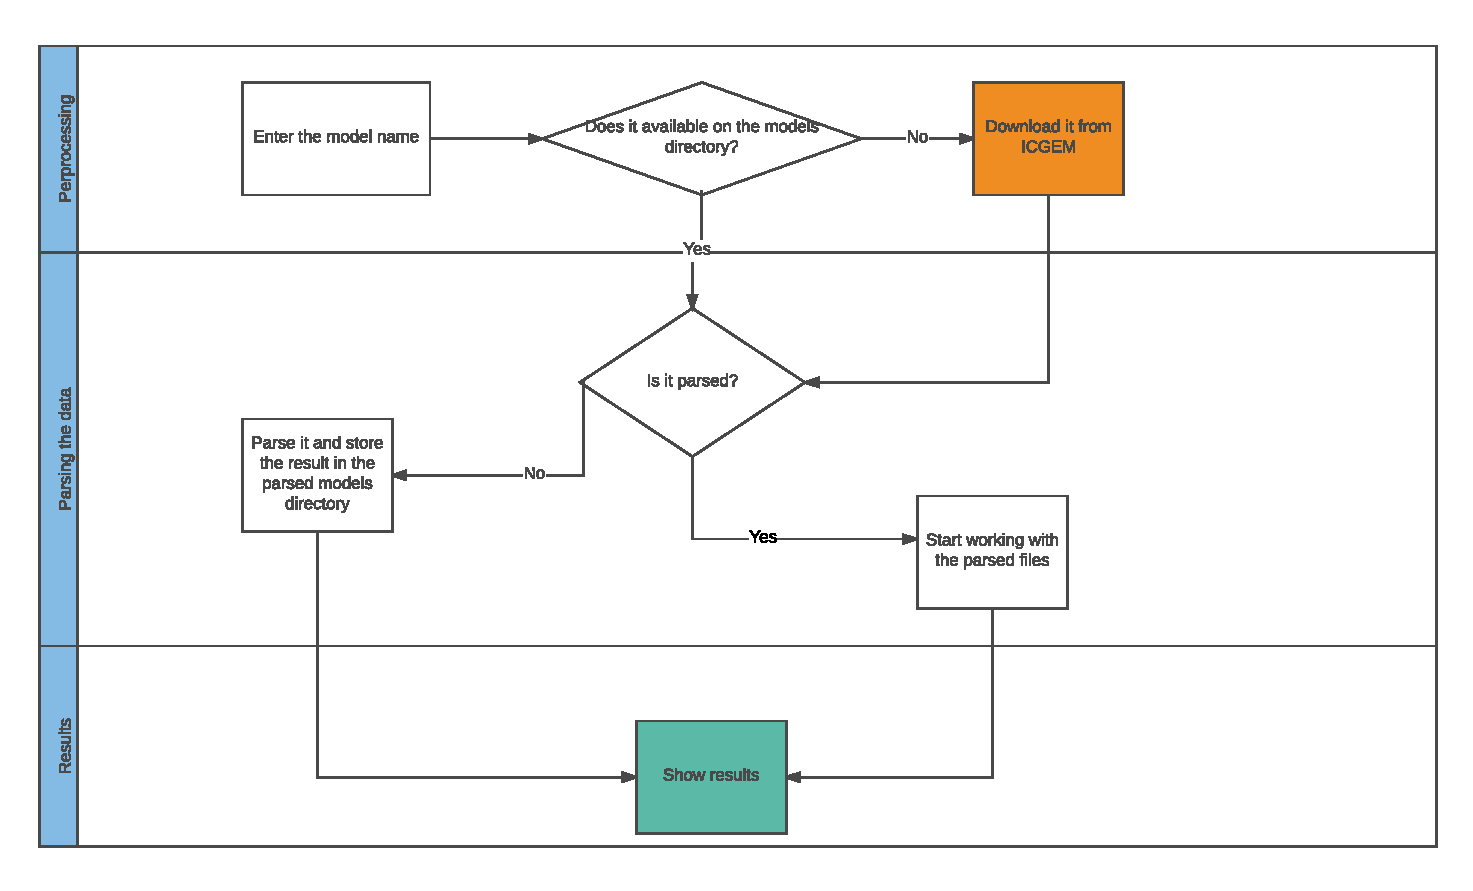
\includegraphics[scale=0.5]{Figures/cropped_final.pdf}
	\centering
\end{figure}

GeoidApp also consists of advanced data analysis tools to help the users get the best out of their models. For each parsed model, GeoidApp creates a directory for that model and stores a log file that logs the result e.g., std and difference, and a *.csv files to store the results in a way that can easily be parsed later. GeoidApp also provides figures for each model being parsed. Another distinct feature is the interactive visualization for the result. This feature comes with the online version of GeoidApp \href{https://geoidapp.github.io}.
\\
The website of GeoidApp has many resources that cover different aspect of GeoidApp. A comprehensive documentation about the application, interactive visualizations, case studies results will all be presented at the website.
 

